% !TEX program = lualatex
\documentclass[lualatex,ja=standard]{bxjsarticle}

\usepackage{tikz}
\usetikzlibrary{arrows.meta}   % 矢印スタイル
\usetikzlibrary{shapes.geometric} % 図形ノード（diamond 等）
\usetikzlibrary{positioning}   % 相対位置指定

\title{TikZ 図形描画のサンプル}
\author{LaTeX サンプル}
\date{\today}

\begin{document}

\maketitle

% -------------------------------------------------------------------
% 基本図形
% -------------------------------------------------------------------
\section{基本図形}

\begin{tikzpicture}
  % 直線
  \draw (0,0) -- (2,0);

  % 矩形
  \draw[blue, thick] (3,0) rectangle (5,1.5);

  % 円
  \draw[red, fill=red!20] (7,0.75) circle (0.75);

  % 楕円
  \draw[green!60!black, fill=green!20] (9.5,0.75) ellipse (1 and 0.5);

  % ラベル
  \node at (1,   -0.4) {直線};
  \node at (4,   -0.4) {矩形};
  \node at (7,   -0.4) {円};
  \node at (9.5, -0.4) {楕円};
\end{tikzpicture}

% -------------------------------------------------------------------
% 矢印・パス
% -------------------------------------------------------------------
\section{矢印・パス}

\begin{tikzpicture}
  % 矢印
  \draw[->, thick]               (0,2)   -- (2,2)   node[right] {->};
  \draw[<->, thick, blue]        (0,1)   -- (2,1)   node[right] {<->};
  \draw[-{Stealth}, thick, red]  (0,0)   -- (2,0)   node[right] {Stealth};

  % 曲線（bezier）
  \draw[->] (4,2) .. controls (5,3) and (6,1) .. (7,2)
    node[right] {ベジェ曲線};

  % 折れ線
  \draw[dashed, orange] (4,0) -- (5,1) -- (6,0) -- (7,1);
\end{tikzpicture}

% -------------------------------------------------------------------
% ノードとラベル
% -------------------------------------------------------------------
\section{ノードと接続}

\begin{tikzpicture}[
  every node/.style={draw, rounded corners, minimum width=2.5cm, minimum height=0.8cm, align=center}
]
  \node (A) at (0,0)   {ノード A};
  \node (B) at (4,0)   {ノード B};
  \node (C) at (2,-2)  {ノード C};

  \draw[->] (A) -- (B) node[midway, above, draw=none] {接続1};
  \draw[->] (A) -- (C) node[midway, left,  draw=none] {接続2};
  \draw[->] (B) -- (C) node[midway, right, draw=none] {接続3};
\end{tikzpicture}

% -------------------------------------------------------------------
% フローチャート
% -------------------------------------------------------------------
\section{フローチャート}

\begin{tikzpicture}[
  start/.style  = {draw, rounded corners=8pt, fill=green!30,  minimum width=2.5cm, minimum height=0.7cm},
  process/.style= {draw, fill=blue!20,        minimum width=2.5cm, minimum height=0.7cm},
  decision/.style={draw, diamond, aspect=2, fill=yellow!30, minimum width=2.5cm},
  stop/.style   = {draw, rounded corners=8pt, fill=red!30,   minimum width=2.5cm, minimum height=0.7cm},
  node distance = 1.2cm
]
  \node[start]    (start)   {開始};
  \node[process,  below=of start]   (proc1)   {処理 A};
  \node[decision, below=of proc1]   (cond)    {条件?};
  \node[process,  below left=of cond, xshift=-0.5cm]  (proc2)   {処理 B};
  \node[process,  below right=of cond, xshift=0.5cm]  (proc3)   {処理 C};
  \node[stop,     below=2.4cm of cond] (stop) {終了};

  \draw[->] (start) -- (proc1);
  \draw[->] (proc1) -- (cond);
  \draw[->] (cond)  -- node[above left]  {Yes} (proc2);
  \draw[->] (cond)  -- node[above right] {No}  (proc3);
  \draw[->] (proc2) |- (stop);
  \draw[->] (proc3) |- (stop);
\end{tikzpicture}

% -------------------------------------------------------------------
% 関数グラフ
% -------------------------------------------------------------------
\section{関数グラフ}

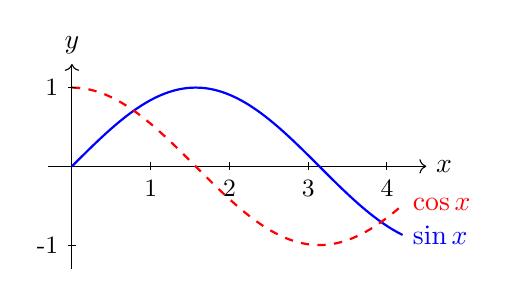
\begin{tikzpicture}
  % 軸
  \draw[->] (-0.3,0) -- (4.5,0) node[right] {$x$};
  \draw[->] (0,-1.3) -- (0,1.3) node[above] {$y$};

  % sin 曲線
  \draw[domain=0:4.2, samples=100, blue, thick]
    plot (\x, {sin(\x r)}) node[right] {$\sin x$};

  % cos 曲線
  \draw[domain=0:4.2, samples=100, red, thick, dashed]
    plot (\x, {cos(\x r)}) node[right] {$\cos x$};

  % 目盛
  \foreach \x in {1,2,3,4}
    \draw (\x, 0.05) -- (\x, -0.05) node[below] {\small\x};
  \foreach \y in {-1,1}
    \draw (0.05,\y) -- (-0.05,\y) node[left] {\small\y};
\end{tikzpicture}

\end{document}